\subsection{sLDS model learns states that correspond to distinguishable behaviors}
\label{sec:slds:3.2.3}
An alternative approach to address jitter in the joint positions would be to use a method that directly incorporates observation noise into the model and can thus learn learn smoothed representations of the observations. The model would then use the smoothed representations to infer the discrete states, thereby avoiding the problem where flickering in the keypoints is absorbed into the model as a state transition. Switching linear dynamical systems (SLDS) models provide a principled way to do precisely that by extending the AR-HMM framework to include an additional layer in between the observations and discrete states (Fig. \ref{fig:slds:3}a). This layer consists of a set of continuous latents that are governed by a Gaussian noise term ($\mathcal{N}(0,Q)$ in Fig. \ref{fig:slds:3}a)), thus acting as a denoised version of the lower-level observations. We write the continuous state update as, 

\begin{equation} \label{eq:slds_3}
x_t = A_{z_t} x_{t-1} + \epsilon \qquad \epsilon \sim \mathcal{N}(0,Q)
\end{equation}
where $x_t$ is the vector of continuous latent states at the current time point, $x_{t-1}$ is the vector of latents at the previous time point, $A$ is a model-inferred dynamics matrix governing how the latents evolve over time in the current discrete state $z_t$, and $\epsilon$ is additive Gaussian noise with covariance $Q$. Note the similarity in structure between Eq. \ref{eq:slds_3} and Eq. \ref{eq:slds_1} in Section \ref{sec:slds:3.2.2}. To connect the continuous latents to the observations we have, 

\begin{equation} \label{eq:slds_4}
y_t = C_{z_t}x_{t} + \nu \qquad \epsilon \sim \mathcal{N}(0,R)
\end{equation}
where $y_t$ is the vector of observations at the current time point, $C$ is a model-inferred loading matrix governing the mapping between the continuous latents and observations for the discrete state at the current time point, and $\nu$ is a noise term with covariance $R$. If the number of continuous latents $p$ is set to be equal to the number of observations $q$, then $C$ will be square and is often enforced to be the identity matrix $I$, thus directly equating each latent to a smoothed version of each observation. However, this setting is not required; even in the case where $C$ is square it does not have to be the identity, and when $p<q$ the continuous latents then serve as a smoothed, lower-dimensional representation of the observations (akin in some ways to performing dimensionality reduction on the observations themselves). As for the discrete state updates, they follow the same formula as the AR-HMM (see Eq. \ref{eq:slds_2}). 

\begin{figure}[t!]
  \begin{center}
    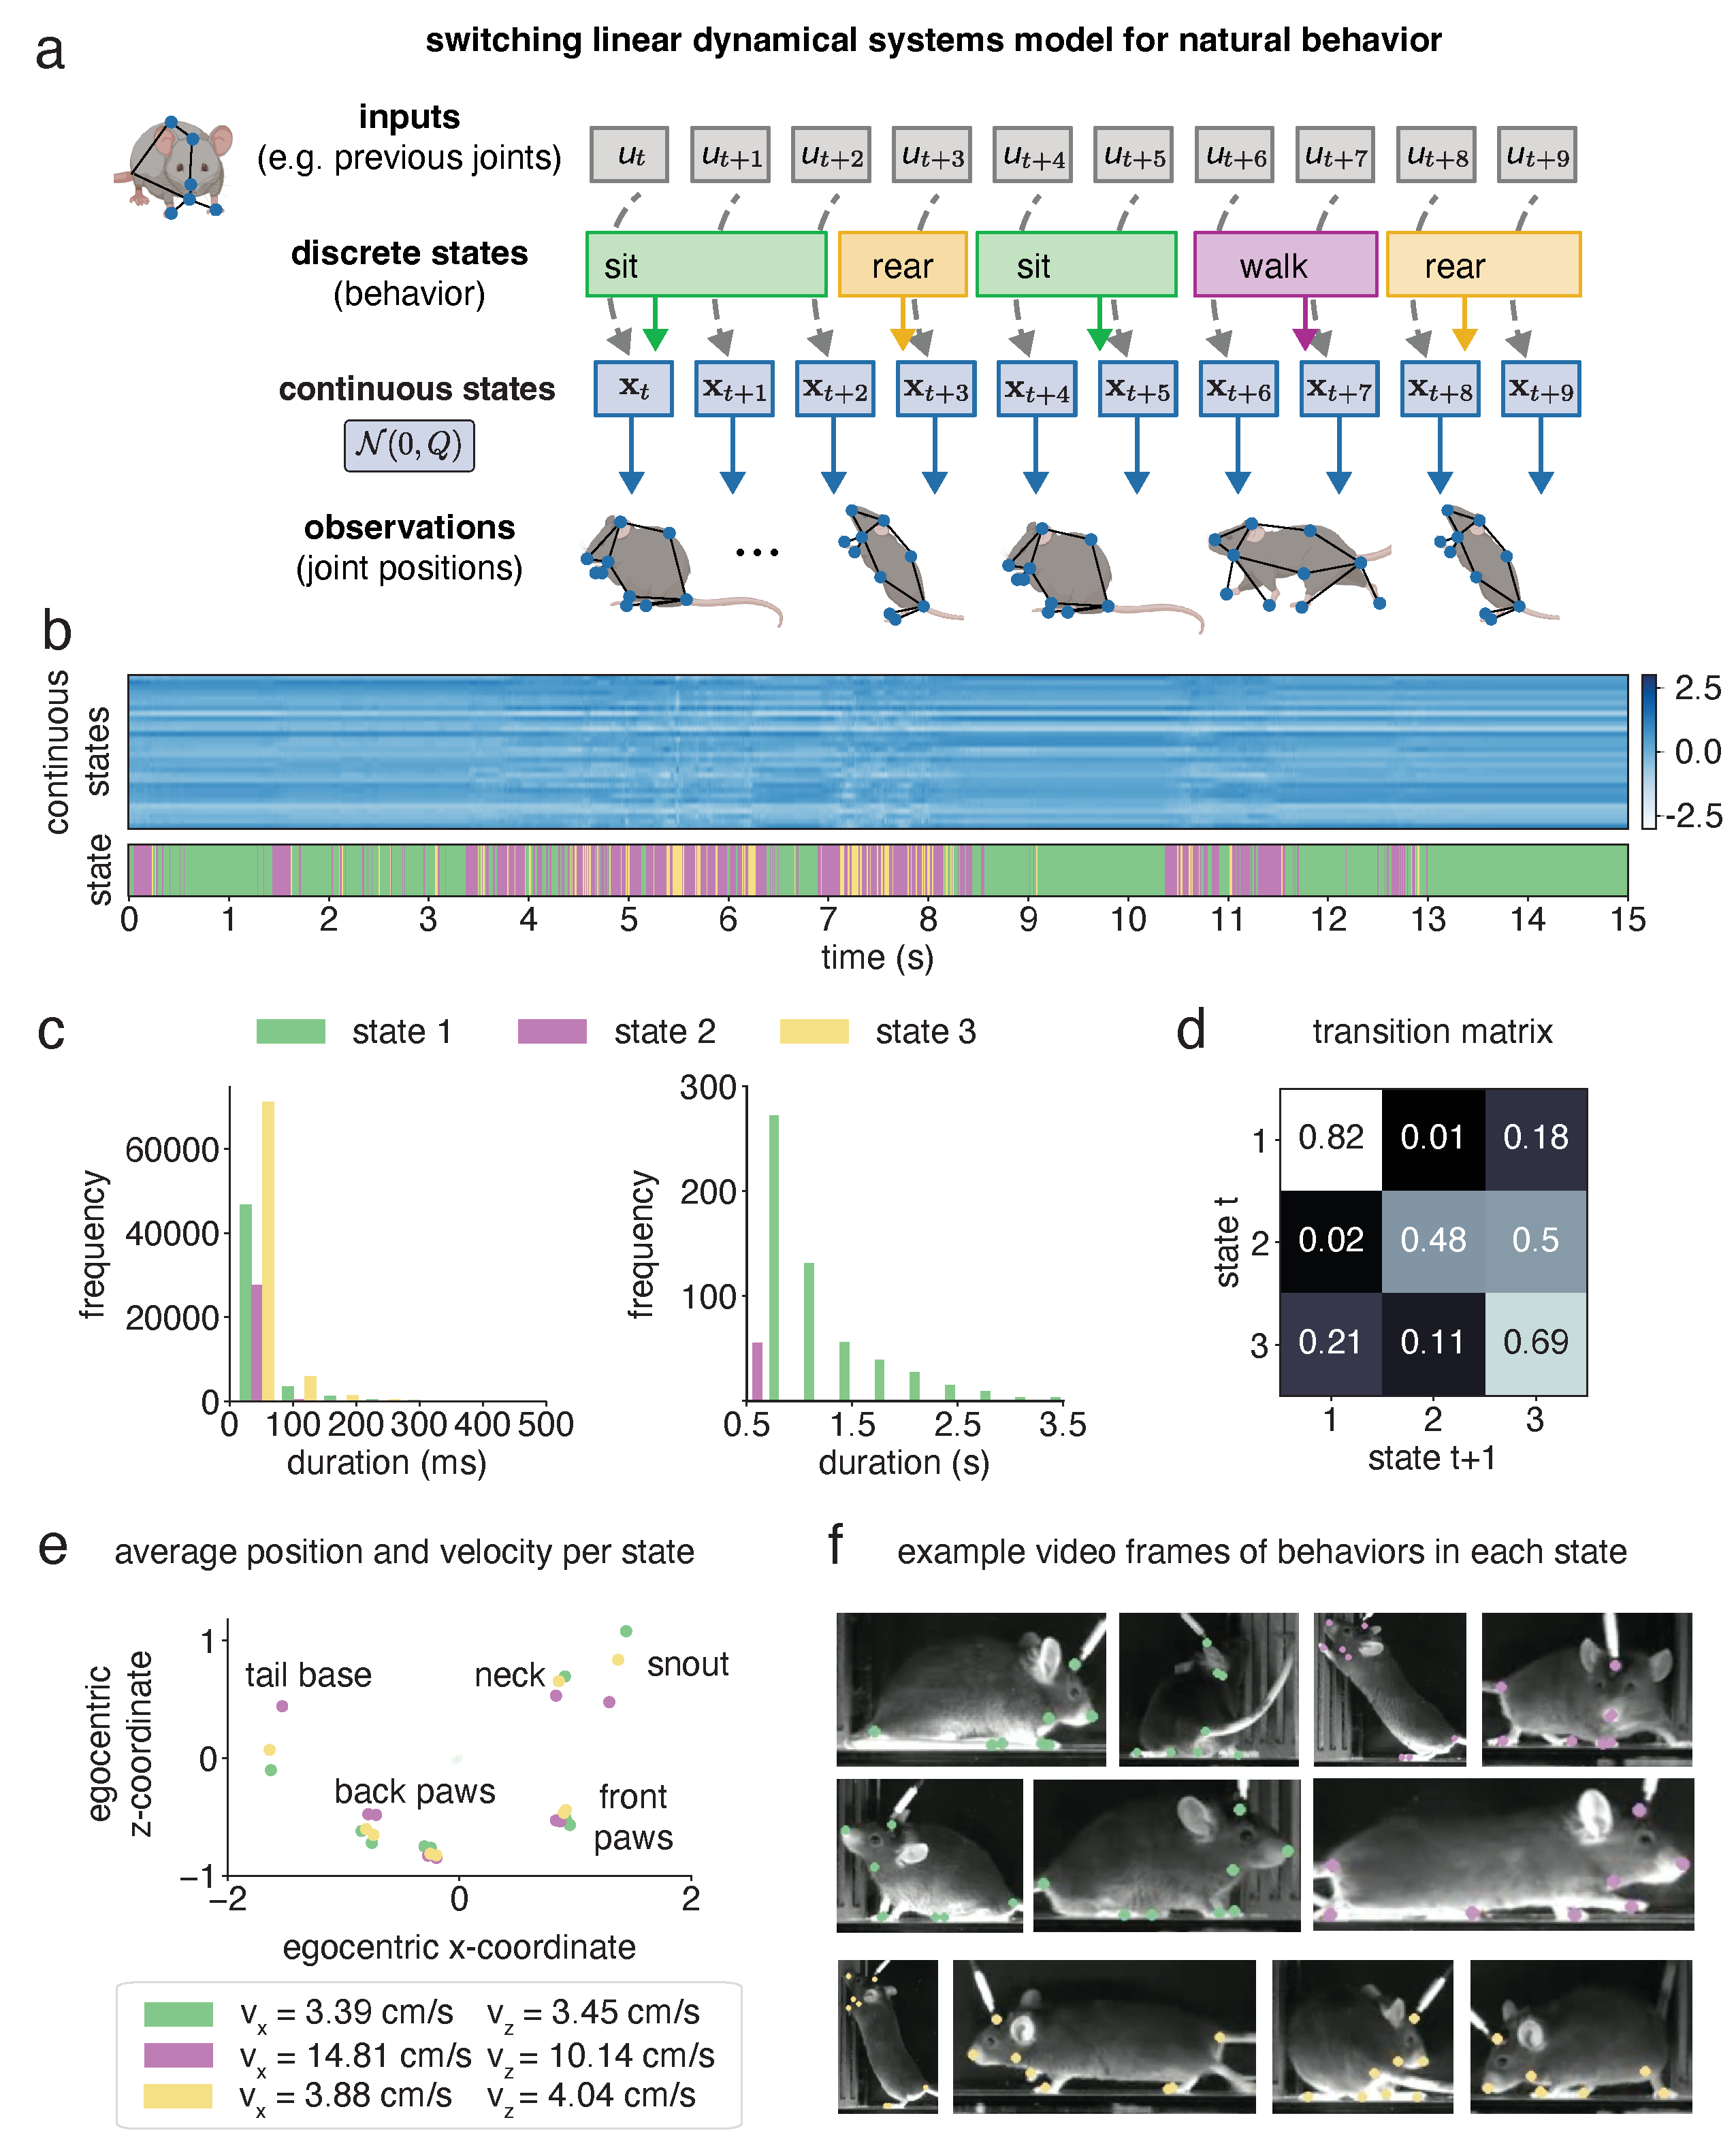
\includegraphics[width=0.90\linewidth]{ch3-slds/slds-figures/Fig3.pdf}
    \caption[SLDS inferred states are longer than AR-HMM inferred states and are more distinguishable in the behaviors they represent]{\textbf{SLDS inferred states are longer than AR-HMM inferred states and are more distinguishable in the behaviors they represent.} (a) SLDS schematic. The model follows the same general structure as the AR-HMM except there is an additional layer of continuous latent states between the discrete states and the observations. (b) Inferred continuous latents (top) with the SLDS inferred most-likely state of the animal at each time point (bottom) for a 15-second time window. (c) Histograms of the state durations for instances of discrete states that last less than 0.5 seconds (left) and greater than 0.5 seconds (right). (d) Discrete state transition probabilities. }
    \label{fig:slds:3}
  \end{center}
  \vspace{-0.5cm}
\end{figure}
\begin{figure}[t!]
  \contcaption{ (e) Average x- and z-positions (length and height view of mouse) of each joint in each state (top) along with per-state average velocities (bottom). (f) Screen grabs of examples of the animals' pose positions in frames the SLDS assigned to each state.}% Continued caption
\end{figure}

We fit a 3-state SLDS to the data with $q=p$ but without requiring $C=I$. Visual inspection of the inferred continuous latents reveals how they act as smoothed representations of the observations (Fig. \ref{fig:slds:3}b, top, compare to Fig. {fig:slds:2}b). The inferred discrete state sequence is also smoother, with long bouts of one state truncated by the other two states in epochs that largely coincide with observable changes in the joint positions (Fig. \ref{fig:slds:3}b, bottom, note in particular the periods between 4-6, 7-8, and 10-12 seconds). This pattern is corroborated by the state duration histograms, which in particular reveal that the model captures long periods of time (up to 3 seconds or longer)  when the animal is in one state, along with average and median state durations 1.38x and 2x longer than the AR-HMM, respectively  (Fig. \ref{fig:slds:3}c, mean=37.2ms, median=20ms). The self-transition probabilities for states two and three are similar to the AR-HMM, whereas state 1 has a substantially higher probability of persisting from one trial to the next (Fig. \ref{fig:slds:3}d). 

The average per-state joint positions and velocities reveal distinct features of the SLDS-inferred states that can be reasonably associated with specific behaviors (\ref{fig:slds:3}e)). The average per-state snout and tail positions are completely non-overlapping, and the neck and back paw positions have partially separated as well. Taken in conjunction with the average per-state velocities in the $x$ and $z$ directions, we can interpret state 1 as a slow-moving state in which the animal's head is relatively high but posterior is low, state 2 as a fast-moving state with even head and posterior positions and raised heels; and state 3 as an intermediate-moving state (particularly in the $z$ direction) in which both snout and tail base tend to be raised. The average per-state durations ($\mu_1$=54.0ms, $\mu_2$=19.2ms, $\mu_3$=32.3ms) indicate that the slow-moving state tends to last the longest, the intermediate state the next longest, and the fast-moving state the shortest, consistent with the results in Fig. \ref{fig:slds:3}c-d. Manual inspection of the videos confirms that state-1 labeled frames tend to correspond to stationary behaviors, whereas states 2 and 3 are more likely to identify non-stationary behaviors of various types, though not always clearly distinguished between walking and rearing. 

